\chapter{Implementation}

This chapter describes the implementation of the codeHelper application. After selecting the technology stack and outlining the system architecture, user interface and workflow, the next stage of development is implementation. The implementation was carried out incrementally, as described in section \ref{sec:designreact}, based on the system requirements in Chapter \ref{chap:req}. 

\section{Client-Server Interaction}

As discussed in the Architectural Design section, section \ref{sec:architecture}, the client-side rendering model requires processing on both the client and server. As discussed in section \ref{sec:architecture}, codeHelper uses a client-server architecture. The interaction between client and server was carried out in two ways - by websockets and HTTP requests.

\subsection{Socket.io}

Socket.IO is a library that enables real-time, bidirectional and event-based communication between the browser and the server \cite{socketio}. Socket.IO is not simply a websocket implementation - it utilises websockets primarily, but can fall back to long-polling when websockets are unavailable. This is useful in our application, since it allows legacy browsers access when websockets are not supported and also an alternative if proxy, firewall or configuration issues prevent a websocket connection from being established.

HTTP long-polling transport, often called long-polling or polling, consists of successive HTTP requests \cite{socketio}. This includes both GET requests for requesting data from the server and POST requests for sending data to the server.

As well as the ability to fallback to long-polling, a key feature of Socket.io is `rooms'. A room is an arbitrary channel that sockets can join and leave that can be used to broadcast events to a subset of clients \cite{socketio}. In the codeHelper system, upon socket connection, users are assigned to rooms. All demonstrators are a member of the `demonstratorChat' room. This allows the tickets and demonstrator messages to be sent exclusively to the demonstrators. Although demonstrators are broadcast all chats in the `demonstratorChat' room (to enable them to interact in every chat via each ticket) each student's chat is broadcast from, and emitted to, the room named for that student. This allows demonstrators to communicate directly with any given student and means that students only have access to their own chat. 

Figure \ref{fig:socketiorooms} shows an example of how rooms are organised in the codeHelper application. \textit{Demonstrator1} is chatting to \textit{student1}, therefore requires access to the `student1' socket room. \textit{demonstrator2} is not chatting to any students and so does not require access to any student socket rooms. Both \textit{demonstrator1} and \textit{demonstrator2} require access to the `demonstratorChat' socket room so that they can receive tickets and demonstratorChat messages. \textit{student1} requires access to the student1 socket so as to receive their associated messages.

\begin{figure}[H]
    \centering
    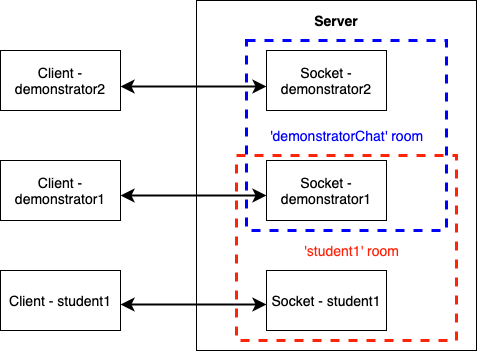
\includegraphics[width=0.6\textwidth]{8implementation/images/socketRooms.png}
    \caption{Example of the organising of Socket.io rooms in the codeHelper application.}
    \label{fig:socketiorooms}
\end{figure}

Socket.io is implemented in the areas of the application where data needs to be real-time. This includes the tickets in the demonstrator help desk, messages, student queue position, messaging and video call initiation. 

The Socket.io connection is established when the user opens the application and the connection is maintained until the application is closed. This is necessary to enable messages to be received whilst the user is at any point in the application. 

\subsection{HTTP Requests}

For data that does not require real-time updates, HTTP requests are used to send and receive data. This includes ticket solutions, summary and statistics data, user roles and student history (i.e. previous tickets).

HTTP requests are made by the client, to the host, which is located on a server. The goal of the request is to access a resource on the server. In order to create the request, the client uses components of a URL (Uniform Resource Locator), which includes the information needed to access the resource \cite{ibmhttp}. 
A HTTP request contains a request line with the request method (GET or POST), the path and the HTTP version. It also contains a series of HTTP headers with information about the message, the sender, and the form of communication. Additionally, a HTTP request can also contain a message body, which includes any input data that the user wishes to send to the server in a POST request \cite{ibmhttp}.

In the codeHelper system, HTTP requests are implemented on the client side using the Fetch API - a standard interface for fetching resources across a network \cite{fetch}. On the server side, the routing and request handling is simplified by using Express \cite{express}, as discussed in section \ref{sec:express}.

POST requests for the creation of, for example, tickets and solutions are sent when the user submits the associated form. GET requests that obtain data for populating pages, such as requesting a solution for a given ticket or requesting a list of all users for the `roles' page, are implemented using the useEffect hook in React \cite{useeffect} - posting the request when the page is accessed, updating the component state with the data and re-rendering the page to show the updated data. This allows page data to be loaded as the page is loaded, providing recent data without the need to manually request as well as reducing the network strain by downloading data only as needed.

\section{Video Calls}

Video calls and screen-sharing were implemented in-app to provide a more complete user experience, as well as to increase efficiency and minimise the surface area of error that is associated with trying to switch between multiple systems (as discussed in section \ref{sec:currentsystem}).

Video calls are implemented using \gls{webrtc}, an open-source project that supports video and voice data to be sent between peers.

The technology is available on all modern browsers and they provide regular Javascript APIs for the technologies behind it, implemented as an open web standard \cite{webrtc}. 

\subsection{PeerJS}

PeerJS is a simple wrapper for the browser's WebRTC implementation. It provides a complete and configurable peer-to-peer connection API which simplifies the browser standard. PeerJS only requires connection to a shared peer server and an ID, with which it can create a \gls{p2p} data or media stream connection to a remote peer \cite{peerjs}.

To facilitate P2P connections, PeerJS connects to a PeerServer. In the codeHelper application, the PeerServer is run on the server. No peer-to-peer data goes through the server, the server acts only as a connection broker \cite{peerjs}. Figure \ref{fig:videoactivity} shows a UML activity diagram for the process of establishing a call between a student and demonstrator using PeerJS, omitting the details of how the PeerServer creates a P2P connection.

\begin{figure}[H]
    \centering
    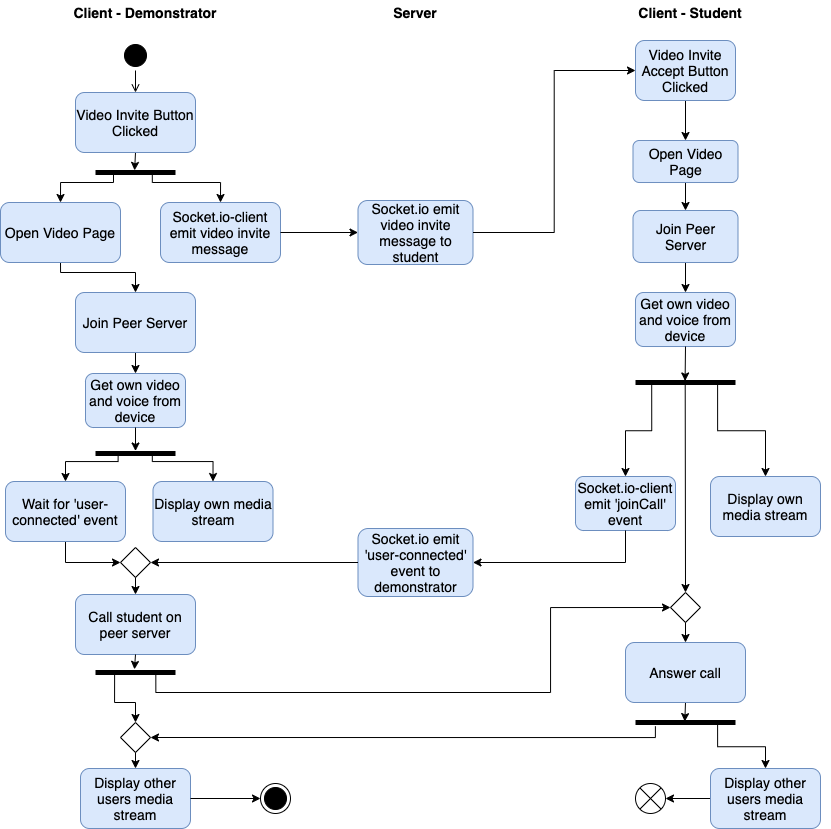
\includegraphics[width=\textwidth]{8implementation/images/activityVideoCall.png}
    \caption{UML activity diagram for a successful video call in the codeHelper application.}
    \label{fig:videoactivity}
\end{figure}

It's important to note that the P2P connection could have been used to send messages but was not. Sending messages over the P2P connection would have improved security, by minimising the risk of messages being misdirected to other users, and improved performance by reducing the traffic and processing carried out on the shared server. However, the application benefited greatly from handling messages separately on the express server since it allows demonstrators to interact with the chats on all tickets. 

\section{File Exchange}

File exchanging was implemented in order to allow students to send image, code or other files in the chat, thereby helping to provide demonstrators with more concrete information that can help them solve the issue.

Files are uploaded to the server using the already established websocket connection. This is implemented using a package called socketio-file-upload \cite{siofu}. A major design choice here was to save the files on the server, rather than to store them temporarily (as with the messages) in the chat. This was done so that demonstrators or lab leads could review files that were exchanged between students and demonstrators.

The chatKey for each chat, corresponding to the room name in Socket.io, is added to the file's meta data. Upon successful upload to the server, the server determines the \gls{mime} type of the object. If the file's MIME type indicates that it is an image, the file is converted to a base 64 string and a message object of type `image' is created and added to the chat - including the image string. This allows the image to be displayed immediately after it is sent. Otherwise, a message of type `file' will be added to the chat, which are rendered on the client side as a hyperlink. For both images and files, clicking on the hyperlink or image will post a HTTP request to the server to download the image based on its file name. Note that if multiple images are uploaded with the same name, socketio-file-upload will rename them and provide that file name to the client.

\section{Database}

The SQL database that was implemented was MariaDB, as discussed in sections \ref{sec:stackdb} and \ref{whysql}. The Node.js package used on the codeHelper server to interact with the database was MySQL2 \cite{npmmysql2}, a drop in replacement for original MySQL package which offers better performance. It was used for this project because of its new implementation of promise wrappers and pooling.

The SQL database originally selected for this project was MySQL, hence the choice of SQL client. The switch to MariaDB did not affect the choice of Node.js package since MariaDB is a drop-in, binary compatible replacement for MySQL \cite{Bartholomew} that works with MariaDB \cite{npmmariadb}.

In the final implementation, a `LoginRequests' table was created to store session information. This resulted in the schema, produced by MySQLWorkbench, show in figure \ref{fig:relationalschemafinal}.

\begin{figure}[H]
    \centering
    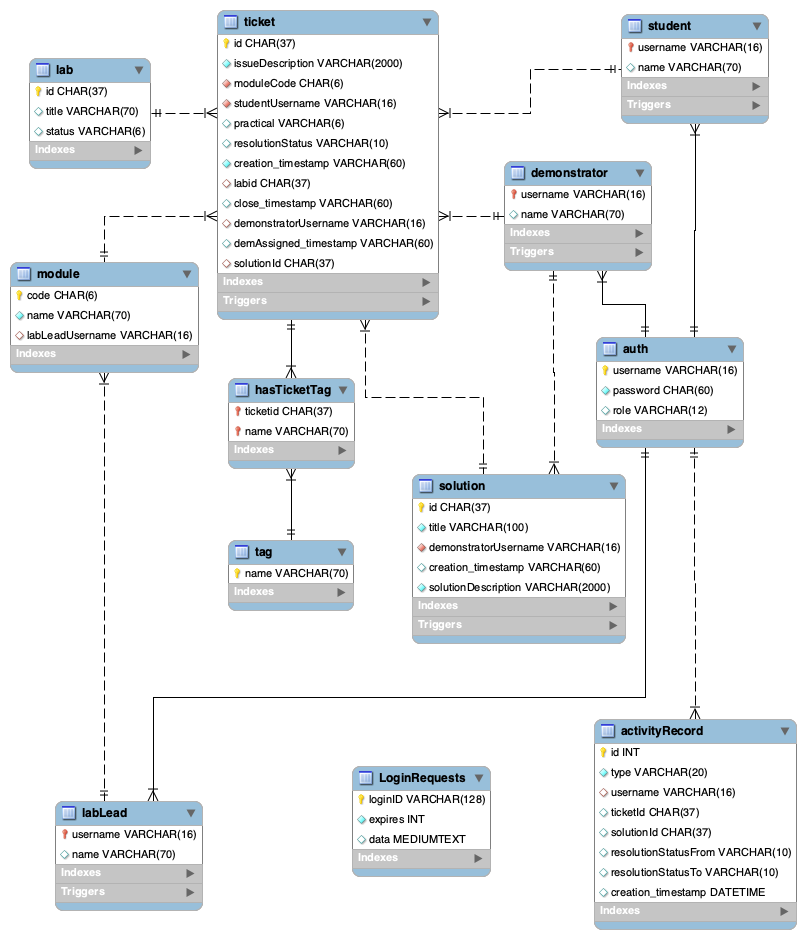
\includegraphics[width=\textwidth]{8implementation/images/schemaFinal.png}
    \caption{Final and complete schema diagram for the system.}
    \label{fig:relationalschemafinal}
\end{figure}

\subsubsection{Triggers}

A trigger is a named database object that is associated with a table, and that activates when a particular event occurs for the table. Some uses for triggers are to perform checks of values to be inserted into a table or to perform calculations on values involved in an update \cite{trigger}. 

Triggers were used for two separate tasks in the building of the codeHelper system.

\paragraph{Recording Activity}
 Triggers were used, upon adding to or editing certain tables, to add activity data to the `activityRecord' table. For example, when a row in the ticket table is updated, one of the triggers shall check if the status of the ticket is the same as it was before the update - if it is not, it shall insert a row into the `activityRecord' table with the value `ticketStatusChanged' in the type column.

\paragraph{Ensuring Demonstrator Privileges} - A trigger is also used to ensure that lab lead accounts also have the privileges of demonstrators. To ensure data consistency, some tables reference the username of users in the demonstrator table. The use of the trigger here allows lab leads to not only perform system administration and view statistics, but also allows them to be able to act as demonstrators in assigning themselves to tickets.

\subsubsection{Attribute Types}
A data type must be specified for each attribute. Table \ref{table:atypetable} below shows the attribute type for each attribute, as well as it's original, parent relational table - in other words, attributes that appear as foreign keys in tables are not repeated.

\begin{table}[H]
\centering
\resizebox{\columnwidth}{!}{%
\begin{tabular}{| c | c | c | c |}
\hline
 Relational Table & Attribute & Attribute Type & Notes\\ 
 \hline
  tag & name & VARCHAR(70) & Government data standards\cite{dataStandards}\\
  \hline
  ticket & ticketId & CHAR(37) & Unique identifier \cite{uuid} prefixed with `T'.\\
  & issueDescription & VARCHAR(2000)&\\
  & practical & VARCHAR(30)& \\
  & resolutionStatus & VARCHAR(10)&[new, missed, inProgress, closed]\\
  & creation\_timestamp & DATE &\\
  &  demAssigned\_timestamp & DATE &\\
  \hline
  solution & solutionId & INT &  Unique identifier \cite{uuid} prefixed with `S'.\\
  & solutionDescription & VARCHAR(2000)&\\
  \hline
  auth & username & VARCHAR(16) & \\
  & password & CHAR(60) & Hashed password. \\
  & role & VARCHAR(12) & [student, demonstrator, labLead] \\
  \hline
  lab & labId & INT& Unique identifier \cite{uuid} prefixed with `L'.\\
  & title & VARCHAR(70) & \\
& status & VARCHAR(6) & [open, closed] \\
  \hline
  user & name & VARCHAR(70)& Government data standards\cite{dataStandards}\\
  \hline
  module & moduleCode & CHAR(6) & Fixed type [A-Z]\{2\}\arraybackslash \textbackslash d\{4\}
\\
  & name & VARCHAR(70)& Government data standards\cite{dataStandards}\\
 \hline
 
 \hline
\end{tabular}}
\caption{Table describing the data types for attributes, showing the parent relational table.}
\label{table:atypetable}
\end{table}

The Government Data Standards Catalogue\cite{dataStandards} was referenced for the data types corresponding to names - including logical extension to category and module names. 

\subsubsection{Data Access Object}

The \gls{dao} pattern was used to create a separation between data access logic and the main application logic. This makes it significantly easier to replace or modify an application's data resources \cite{daooracle} that may arise in future refactoring or adaptation. 

There are three key benefits to implementing the use of a DAO \cite{daooracle}:

\begin{itemize}
    \item Separation of the data resource's client interface from its data access mechanisms
    \item Adapation of a specific data resource's access API to a generic client interface
    \item Allowing data access mechanisms to change independently of the rest of the system
\end{itemize}

\section{Authentication}

Authentication in the application is implemented using PassportJS, an authentication middleware for Node which authenticates requests. 

\subsection{PassportJS}

In Passport, a `local' strategy was used, meaning Passport verifies user credentials against a store of users in the database. Implementation of Passport allows the system to be adapted for the use of different strategies - including single sign-on using an OAuth provider such as Facebook or Twitter, both of which have become popular authentication methods \cite{passport}. 

\subsubsection{HTTP Requests}

\begin{figure}[H]
    \centering
    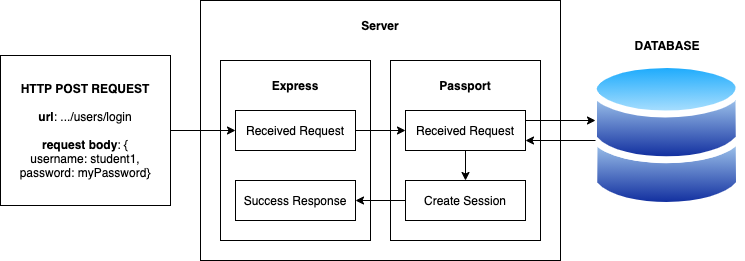
\includegraphics[width=\textwidth]{8implementation/images/passport.png}
    \caption{Basic flow of data for login using Passport.}
    \label{fig:passportlogin}
\end{figure}

Figure \ref{fig:passportlogin} shows an extremely simplified version of the basic flow of data for a user who logs in using Passport. The following steps are carried out when a user attempts to login:
\begin{enumerate}
    \item The user submits the login form, sending a HTTP POST request to .../users/login with the username and password contained in the request body.
    \item The passport.authenticate middleware is called, verifying the user by checking the user's posted credentials against the encrypted credentials stored in the database.
    \item Passport.authenticate passes the user (with hashed password) object, along with any errors or additional info (if added).
    \item If the authentication was passed, Passport will automatically log the user in by calling req.login - a functino that passport has attached to the object express uses to represent the HTTP request.
    \item Passport will use the custom serialize function to attach data to request object, in our case only the user's username.
    \item Express sends a response with status 200 the username, role and message - or, if not authenticated, a 401 response with an invalid credentials message.
\end{enumerate}

For any further requests:

\begin{enumerate}
    \item Express accesses the session data in the database and attaches it to the request. Passport is able to access the serialised user object in the request.
    \item Passport.session is invoked, checking for a serialised user object in the session.
    \item Passport.session calls the custom deserialise function, finding the user and passing them to the next middleware - it acts as a middleware which takes the request object and converts the session id (from the client cookie) into the true deserialized user object that was specified.
    \item A custom middleware function checks that the user has the required role to access the API endpoint by checking the deserialized user object.
\end{enumerate} 

\subsubsection{Socket.io}

The Websockets also implement Passport JS as a middleware, in the same way as HTTP requests do shown in figure \ref{fig:passportlogin}. 

Further, misuse by students in Socket.io is prevented by not reading the `chat' argument sent by students - whereas demonstrators specify the chat so as to be able to participate in multiple conversations. For example, when a chat message is sent to the server it has the properties `text' (containing the message text) and `chat' (specifying which chat the message is sent to) - however the chat property is only read if the user is not a student. See figure \ref{fig:socketchat}.

\begin{figure}[H]
    \centering
    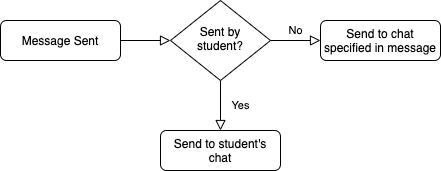
\includegraphics[width=0.7\textwidth]{8implementation/images/socketiochat.png}
    \caption{Flowchart describing logic for processing incoming chats.}
    \label{fig:socketchat}
\end{figure}

This works because students have access to, and are associated with, only their own chat, whereas demonstrators can interact with any student chat.

Additionally, Passport JS is used to authenticate socket connection requests and to assign socket usernames. The basic process is shown in figure \ref{fig:socketpassport}. By authenticating Socket.io connections with passport, the authentication of the codeHelper application is consistent. The original implementation followed the same process for setting a username as online documentation \cite{socketpassport}, by attaching the username as meta data on the socket request. The revised method of setting usernames on the server side is more secure, as it prevents users from `listening' to data on others' socket connections - which could include all of the application's tickets and messages.

\begin{figure}[H]
    \centering
    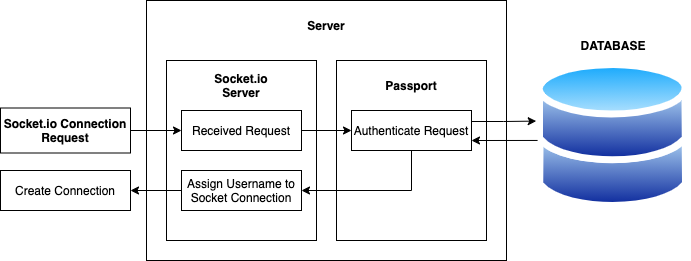
\includegraphics[width=\textwidth]{8implementation/images/socketPassport.png}
    \caption{Process of authenticating websocket connection and assigning username.}
    \label{fig:socketpassport}
\end{figure}